\documentclass[12pt]{article}

\usepackage{verbatim}
\usepackage{listings}
\usepackage{color}
\usepackage{graphicx}
\usepackage{amsmath}


%%
\title{Probleme: Mesure nombre de tour d'une bobine}

\author{Fabien Le Mentec\\
\small \texttt{texane@gmail.com}
}

\date{}

\begin{document}
\maketitle

%%
\newpage
\begin{abstract}
Dans le cadre du projet, on cherche a soulever un aimant grace a la force
du champs magnetique produit par un courant passant dans une bobine. On veut
mesurer le nombre de tours de bobine necessaires.
\end{abstract}

%%
\newpage
\section{Description du probleme}
\paragraph{} La figure suivante schematise le probleme:
\begin{center}
  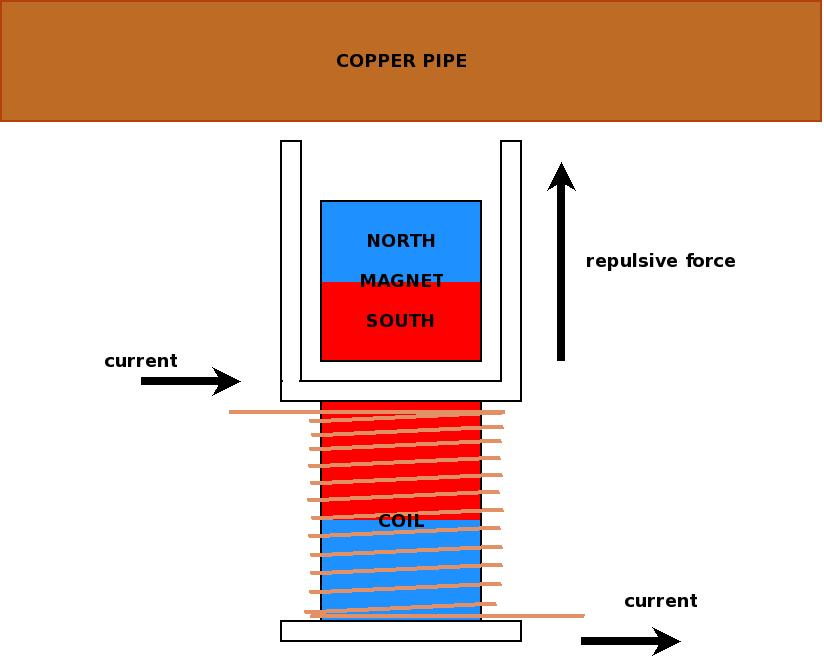
\includegraphics[keepaspectratio=true, width=65mm]{dia/coil/coil.jpg}\\
\end{center}

\paragraph{} On dispose des informations suivantes:
\begin{itemize}
  \item aimant
    \begin{itemize}
    \item hauteur: $10mm$
    \item diametre: $8mm$
    \item densite: $7.5g./cm^{3}$
    \end{itemize}

  \item bobine
    \begin{itemize}
    \item fil de cuivre emaille, diametre: $0.20mm$
    \item diametre de la bobine: $< 30mm$
    \item hauteur de la bobine: $< 30mm$
    \end{itemize}  

  \item alimentation
    \begin{itemize}
    \item DC 5 volts
    \end{itemize}
\end{itemize}

\paragraph{} On cherche a savoir le nombre de tours de bobine necessaires
pour soulever l'aimant d'une distance superieure ou egale a 5mm.

\end{document}
